\documentclass{article}
\usepackage[a4paper, margin=3mm, landscape]{geometry}
\usepackage{multicol}
\usepackage{xcolor}
\usepackage{enumitem}
\usepackage{amsmath}
\usepackage{amsfonts}
\usepackage{listings}
\usepackage{soul}
\usepackage{graphicx}

\pdfinfo{
    /Title (GEC1010.pdf)
    /Creator (TeX)
    /Producer (pdfTeX 1.40.0)
    /Author (Vincent Pang)
    /Subject (GEC1010)
    /Keywords (GEC1010, nus, cheatsheet, pdf)
}

\graphicspath{ {./img/} }

\pagestyle{empty}
\setcounter{secnumdepth}{0}
\setlength{\columnseprule}{0.25pt}

% Redefine section commands to use less space
\makeatletter
\renewcommand{\section}{\@startsection{section}{1}{0mm}%
    {-1ex plus -.5ex minus -.2ex}%
    {0.5ex plus .2ex}%x
{\normalfont\large\bfseries}}
\renewcommand{\subsection}{\@startsection{subsection}{2}{0mm}%
    {-1explus -.5ex minus -.2ex}%
    {0.5ex plus .2ex}%
{\normalfont\normalsize\bfseries}}
\renewcommand{\subsubsection}{\@startsection{subsubsection}{3}{0mm}%
    {-1ex plus -.5ex minus -.2ex}%
    {1ex plus .2ex}%
{\normalfont\small\bfseries}}%
\makeatother

% Adjust spacing for all itemize/enumerate
\setlength{\leftmargini}{0.5cm}
\setlength{\leftmarginii}{0.5cm}
\setlist[itemize,1]{leftmargin=2mm,labelindent=1mm,labelsep=1mm}
\setlist[itemize,2]{leftmargin=2mm,labelindent=1mm,labelsep=1mm}

% Font
\renewcommand{\familydefault}{\sfdefault}

% Define colors for math formulas
\definecolor{myblue}{cmyk}{1,.72,0,.38}
\everymath\expandafter{\the\everymath \color{myblue}}

% Custom command for keywords
\definecolor{highlight}{RGB}{251,243,218}
\newcommand{\keyword}[2][]{\sethlcolor{highlight}\hl{\textbf{#2}} #1 - }
\newcommand{\ilkeyword}[1]{\sethlcolor{highlight}\hl{\textbf{#1}}}

% Define colors and style for code
\definecolor{codegreen}{rgb}{0,0.6,0}
\definecolor{codegray}{rgb}{0.5,0.5,0.5}
\definecolor{codered}{HTML}{CC241D}
\definecolor{backcolor}{rgb}{0.95,0.95,0.95}
\lstdefinestyle{codestyle}{
    backgroundcolor = \color{backcolor},
    commentstyle = \color{codegray},
    keywordstyle = \color{codered},
    stringstyle = \color{codegreen},
    basicstyle = \ttfamily,
    breakatwhitespace = false,
    showstringspaces = false,
    breaklines = true,
    showtabs = false,
    tabsize = 2
}
\lstset{style = codestyle}

% -----------------------------------------------------------------------
\begin{document}
\begin{multicols*}{3}
\footnotesize

% Title box
\begin{center}
    \fbox{
        \parbox{0.8\linewidth}{
            \centering \textcolor{black}{
                {\Large\textbf{GEC1010}} \\
                \normalsize{AY22/23 Sem 2}} \\
                {\footnotesize \textcolor{gray}{github.com/securespider}}
        }
    }
\end{center}
\section{01. Energy}
\subsection{By constant force}
work done by a force == force * displacement
\\$W = FS$
\subsection{Law of conservation of energy}
Energy can neither be created nor destroyed, it can only be transformed from one form to another
\subsection{Kinetic energy}
Formula in linear motion\\
$K=\dfrac{1}{2}mv^2$\\
Formula in angular motion\\
$\dfrac{1}{2}I\omega^2$\\
\begin{itemize}
	\item I = Moment of inertia of object (dependent on mass distribution of object)
	\item $\omega$ = angular velocity of the rotating object
	\begin{itemize}
		\item Rad/second
		\item $v = \omega * radius$
	\end{itemize}
\end{itemize}
\subsection{Gravitational potential energy}
$U = mgh$

\subsection{Power}
Rate of doing work or rate of consumption of energy\\
$P = \dfrac{\triangle W}{\triangle t}$\\
Work done, W, by a system in time t

\subsection{Requirements of an energy system}
\subsubsection{Energy resource}
\begin{itemize}
	\item Clean energy 
	\begin{itemize}
		\item Wind Energy
		\item \keyword{Hydro energy}{Come from river and dams}
		\item Ocean energy{Only refers to energy coming from ocean currents etc}
		\item Solar energy
		\item Biomass
		\item Non-Renewables:
		\item Geothermal
		\item Nuclear
	\end{itemize}
	\item Fossil fuels
	\begin{itemize}
		\item Coal
		\begin{itemize}
			\item Greater carbon content and more impurities - More carbon dioxide and greater air pollution
			\item Solid so difficulty in extraction, transportation and use
			
		\end{itemize}
		\item Natural Gas
		\begin{itemize}
			\item Cleaner alternative 
		\end{itemize}
		\item Oil
	\end{itemize}
\end{itemize}	
Problems
\begin{itemize}
	\item Unsustainable - reserves depleting
	\item Global warming - Enhanced greenhouse effect by earth atmosphere
	\item Greater absorption of long wavelength IR in earth's atmosphere
	\item Rising temperature anomaly from 1980-2000	
	\item Global sea level rising
	\begin{itemize}
		\item Thermal expansion of water
		\item Melting alpine glaciers and ice sheets
	\end{itemize}
	\item Earlier timing of spring events
	\item Poleward and upward shift in plant and animal species
\end{itemize}
Solution:\\
Clean energy
\begin{itemize}
	\item Replace existing supply of fossil fuels
	\item Use energy more efficiently and judiciously minimizing environmental pollution
\end{itemize}
\subsubsection{High power}
\subsubsection{High energy conversion efficiency}
\subsection{Singapore}
Singapore uses LNG primarily (95\%) piped from indonesia and malaysia\\
Switching to solar and biofuels to reduce reliance
\subsubsection{Energy conservation}
\begin{itemize}
	\item Outdoor LED initative
	\item Electric car sharing
\end{itemize}

% -----------------------------------------------------------------------

\section{02. Fundamentals of thermal energy}
$Q=mc\triangle T$
\begin{description}
	\item[Q]{Heat energy supplied}
	\item[m]{mass}
	\item[c]{Specific heat capacity of material}
	\item[T]{temperature change resulting from heat energy}
\end{description}
$Q=mL$
\begin{description}
	\item[Q]{Heat energy supplied}
	\item[m]{mass}
	\item[L]{Specific latent heat of vaporization/fusion}
\end{description}

\subsection{Types}
\begin{itemize}
	\item Conduction
	\begin{itemize}
		\item Dominant in solids
	\end{itemize}
	\item Convection
	\begin{itemize}
		\item Dominant in fluids (liquid and gases)
		\item Works by circulating fluids and thermal expansion properties of materials
		\item Cold fluids sink, warm fluid rise
	\end{itemize}
	\item Radiation
\end{itemize}

\subsection{Stefan Boltzmann Law}
Power of black body radiation\\
$P = \epsilon\sigma T_0^4$
\begin{enumerate}
	\item[P]{Energy absorbed per unit second per unit area via radiation}
	\item[$\epsilon$]{Emissivity of surface(lies between 0-1)}
	\item[$\sigma$]{$5.67*10^{-8}$ = Stefan Boltzmann constant}
\end{enumerate}


% -----------------------------------------------------------------------
% -----------------------------------------------------------------------
% -----------------------------------------------------------------------
% -----------------------------------------------------------------------
% -----------------------------------------------------------------------

\section{05. Hydro power}
\subsection{Ocean vs River}
River
\begin{enumerate}
	\item Hydroelectricity
\end{enumerate}
Ocean
\begin{enumerate}
	\item Tidal power
	\item Wave power
	\item Ocean thermal
\end{enumerate}
\subsection{Water wheels}
\subsubsection{Water mills}
\begin{itemize}
	\item Ancient application for replacing physical labour
	\item Replaced with water turbines for energy generation
\end{itemize}
Types of water wheels\\
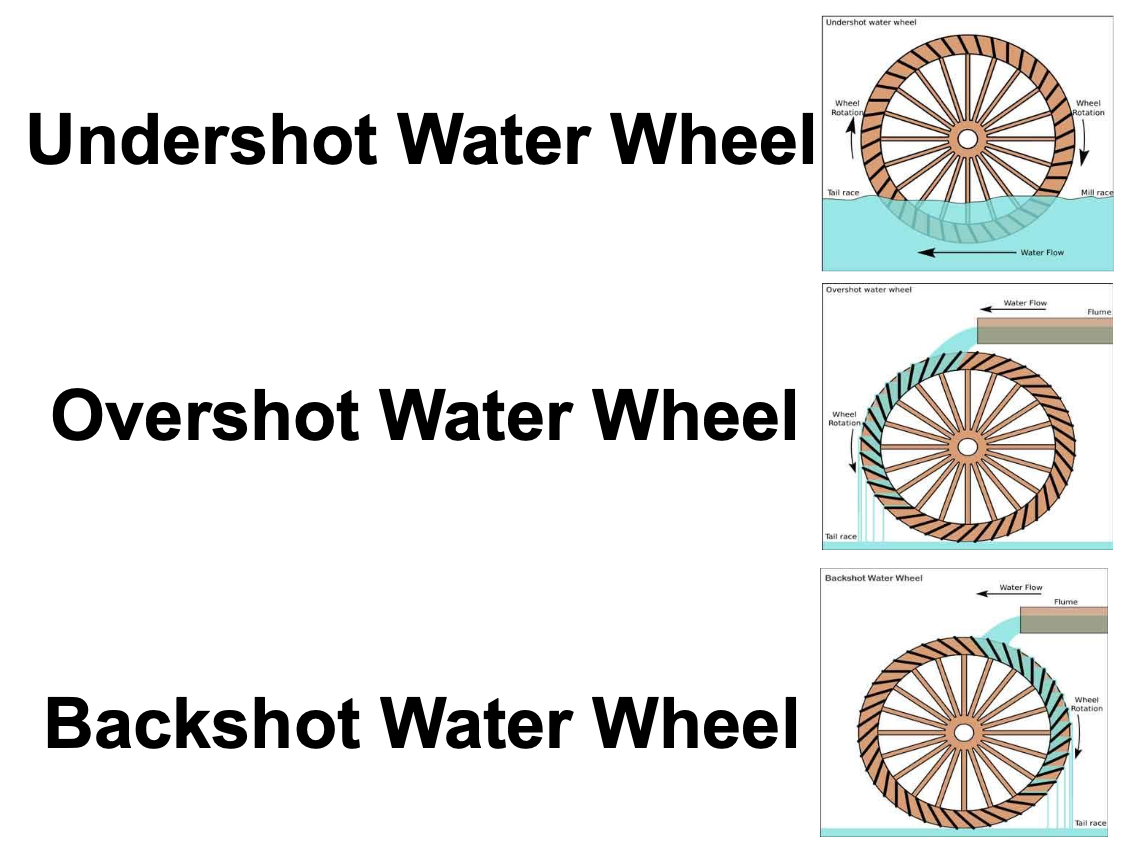
\includegraphics[scale=0.3]{water-wheels}
\begin{itemize}
	\item Undershot
	\begin{itemize}
		\item Vertically mounted with water flowing at the bottom of the wheel
		\item Cheapest and least efficient
	\end{itemize}
	\item Overshot
	\begin{itemize}
		\item Falling water on the top of the wheel in direction of rotation
		\item Use all water flow for power production 
		\item Does not require rapid flow of water
		\item Uses the difference in weight between the 2 sides of the wheel to turn
	\end{itemize}
	\item Backshot
	\begin{itemize}
		\item Introduced behind the apex of the wheel
		\item Water flows opposite the direction of rotation
		\item Continues to function even when water in wheel put rises beyond height of axle
		\item Technique useful for streams that experience extreme seasonal variations in flow
	\end{itemize}
\end{itemize}

\subsection{Types of Hydro Power}
\begin{itemize}
	\item Dam based
	\item Run of the river plants(diversion)
	\item Pumped storage technology
	\item Damless hydro power
\end{itemize}
\subsubsection{Principles of power generation}
Production of electricity by using gravitational force of falling water\\
$P=\eta\rho ghQ$\\
$\eta$ = efficiency, $\rho$ = density of water, Q = Volume of water flowing per second on turbine, h = Vertical distance between turbine and water surface

\end{multicols*}
\end{document}
